%; whizzy chapter -dvi
% -initex iniptex -latex platex -format platex -bibtex jbibtex -fmt fmt
% 以上 whizzytex を使用する場合の設定。
 
%     Tokyo Debian Meeting resources
%     Copyright (C) 2012 Junichi Uekawa
%     Copyright (C) 2011 Nobuhiro Iwamatsu

%     This program is free software; you can redistribute it and/or modify
%     it under the terms of the GNU General Public License as published by
%     the Free Software Foundation; either version 2 of the License, or
%     (at your option) any later version.

%     This program is distributed in the hope that it will be useful,
%     but WITHOUT ANY WARRANTY; without even the implied warranty of
%     MERCHANTABILITY or FITNESS FOR A PARTICULAR PURPOSE.  See the
%     GNU General Public License for more details.

%     You should have received a copy of the GNU General Public License
%     along with this program; if not, write to the Free Software
%     Foundation, Inc., 51 Franklin St, Fifth Floor, Boston, MA  02110-1301 USA

%  preview (shell-command (concat "evince " (replace-regexp-in-string "tex$" "pdf"(buffer-file-name)) "&"))

%%ここからヘッダ開始。

\documentclass[mingoth,a4paper]{jsarticle}
\usepackage{monthlyreport}

% 日付を定義する、毎月変わります。
\newcommand{\debmtgyear}{2013}
\newcommand{\debmtgmonth}{11}
\newcommand{\debmtgdate}{16}
% started from zero:
% (let ((year 2013) (month 7)) (+ (* (- year 2005) 12) month -1))
\newcommand{\debmtgnumber}{106}

\begin{document}

\begin{titlepage}
\thispagestyle{empty}
% タイトルページ:編集必要な部分は最初のマクロに飛ばすこと

\vspace*{-2cm}
第\debmtgnumber{}回 東京エリア Debian 勉強会資料\\
\hspace*{-2cm}

\includegraphics{image2012-natsu/dotdeb.pdf}\\
\hfill{}\debmtgyear{}年\debmtgmonth{}月\debmtgdate{}日

% ここはアップデートすること
% 全角文字にしないとフォントのサイズが合わないので注意
\rotatebox{10}{\fontsize{32}{32} {\gt 特集1: waylandを動かす}}

\rotatebox{10}{\fontsize{32}{32} {\gt 特集2: tramp環境構築}}

\vspace*{-2cm}
\hfill{}
\includegraphics[height=6cm]{image200502/openlogo-nd.eps}
\end{titlepage}

\newpage

\begin{minipage}[b]{0.2\hsize}
 \definecolor{titleback}{gray}{0.9}
 \colorbox{titleback}{\rotatebox{90}{\fontsize{80}{80} {\gt デビアン勉強会} }}
\end{minipage}
\begin{minipage}[b]{0.8\hsize}
\hrule
\vspace{2mm}
\hrule
\begin{multicols}{2}
\tableofcontents
\end{multicols}
\vspace{2mm}
\hrule
\end{minipage}

\dancersection{事前課題}{上川 純一}

今回の事前課題は以下です:
\begin{enumerate}
 \item wayland vs mir についておもうことを語ってください。
\end{enumerate}
この課題に対して提出いただいた内容は以下です。
\begin{multicols}{2}
{\small
 
\begin{prework}{ $BLn<s(B }

$B8eH/$G$"$j$J$,$iM%0L@-$N$_$i$l$J$$(BMir$B$K0UL#$,$"$k$H$9$l$P!"$=$l$O(BCanonical$B$,%3%s%H%m!<%k2DG=$JE@$@$1$J$N$+$J$H$$$&5$$,$7$^$9!#(B

\end{prework}

\begin{prework}{ dictoss($B?yK\!!E5=<(B) }


\end{prework}

\begin{prework}{  $B@6LnM[0l(B }

$BIaCJ$"$^$j0U<1$7$?$3$H$,$J$+$C$?$N$G!"$3$l$r5$$KJY6/$G$-$l$P$H;W$$$^$9!#(B
\end{prework}

\begin{prework}{ mtoshi }

$B$5$C$Q$jJ,$+$j$^$;$s(B($BN^(B)
\end{prework}

\begin{prework}{ $B$^$($@$3$&$X$$(B }

$BL>A0$7$+<*$K$7$?$3$H$,$J$$$N$G!"$5$C$Q$jJ,$+$i$J$$!#(B
\end{prework}

\begin{prework}{ $BLnEg!!5.1Q(B }

wayland$B$b4hD%$C$?!*(Bmir$B$O<+J,$O$h$/$o$+$i$s$,!"4hD%$C$F$k!*(BX$B$bIi$1$F$J$$!*(B
$B$$$d!<!"$3$A$i$N@o$$$OL\$,$O$J$;$^$;$s%M!<!#2?;v$b6%AhAj<j$,$$$k$C$FNI$$$3$H$G$9%M!<!#(B
mir$B$H$NHf3S$O8!F$$7$?$3$H$J$$$N$G!"0c$$$K$D$$$FC/$+$h$m$7$/$*$M$,$$$7$^$9!#$$$:$l$K$7$F$b!"<+J,$H$7$F$O!"AH$_9~$_4^$a$F4JC1$KM7$Y$=$&$@$7!"Cf?H$9$C$4$$$o$+$j$d$9$$<BAu$G$"$k!"(Bwayland$B$H$7$P$i$/5:$l$h$&$H;W$C$F$^$9!#(B

$B"((Bmir$B$OD4$Y$F$J$$$h(B?

\end{prework}

\begin{prework}{ $B>e@n=c0l(B }

x11$B$N%W%m%H%3%k$O2~NI$NM>CO$,$"$k$H;W$&$N$G4hD%$C$F3+H/$,?J$_6%Ah$,$"$k$N$O9%$^$7$$$H;W$$$^$9!#(B
\end{prework}

}
\end{multicols}

\dancersection{Debian Trivia Quiz}{上川純一}

ところで、みなさん Debian 関連の話題においついていますか?Debian関連の話
題はメーリングリストをよんでいると追跡できます。ただよんでいるだけではは
りあいがないので、理解度のテストをします。特に一人だけでは意味がわからな
いところもあるかも知れません。みんなで一緒に読んでみましょう。

今回の出題範囲は\url{debian-devel-announce@lists.debian.org} や \url{debian-devel@lists.debian.org}に投稿された
内容などからです。

\begin{multicols}{2}
 %; whizzy-master ../debianmeetingresume201311.tex
% $B0J>e$N@_Dj$r$7$F$$$k$?$a!"$3$N%U%!%$%k$G(B M-x whizzytex $B$9$k$H!"(Bwhizzytex$B$,MxMQ$G$-$^$9!#(B
%

\santaku
{alioth $B$K$J$K$,$*$-$?$+(B}
{$B7|>^$,$"$?$C$?(B}
{RAID$B$N%O!<%I%G%#%9%/$,(B2$B8D2u$l$?(B}
{$B?7%"!<%-%F%/%A%c$K0\9T$7$?(B}
{B}
{RAID$B$N%O!<%I%G%#%9%/$,(B2$B$D2u$l$F%U%!%$%k%7%9%F%`$,2u$l$?$=$&$G$9!#(B}

\santaku
{DSA$B$,(BDPL$B$N>5G'$J$/;H$($kM=;;$O$$$/$i$+(B}
{\$ 0}
{\$ 100}
{\$ 400}
{C}
{$B%G%#%9%/$,2u$l$F8r49$9$k$N$K$b(BDPL$B$r$^$?$J$$$H$$$1$J$+$C$?$N$+$J!#(B}

\santaku
{Jessie $B$N%U%j!<%:$O$$$D$+(B}
{2013$BG/(B11$B7n(B5$BF|(B}
{2014$BG/(B11$B7n(B5$BF|(B}
{2015$BG/(B11$B7n(B5$BF|(B}
{A}
{$B$"$l!"$b$&%U%j!<%:$7$F$k!)(B}

\santaku
{policy 3.9.5.0$B$K$h$k$H%P%$%J%j%Q%C%1!<%8Fb$N%U%!%$%kL>$N%(%s%3!<%G%#%s%0$O$J$K$+(B}
{UTF-8}
{Latin-1}
{sjis}
{A}
{$B$H$&$H$&(BASCII$B0J30$,G'$a$i$l$k$h$&$K$J$j$^$7$?$+!#(B}

\end{multicols}

% \dancersection{最近のDebian関連のミーティング報告}{上川純一}
% \subsection{東京エリアDebian勉強会103回目報告}

% \subsection{OSC 東京/Fall}


% % (query-replace-regexp "<.*?>" "")
% % (query-replace-regexp "^[	 ]\+" "")

%-------------------------------------------------------------------------------
\dancersection{waylandを動かす}{野島 貴英}
%-------------------------------------------------------------------------------
\index{wayland}

\subsection{wayland}
 waylandとは、Kristian H\o{}gsbergさんが中心となって作っているディスプレイサーバーのプロトコルのことです。waylandプロトコルを扱えるディスプレイサーバーとしてwestonがあります。 
\index{weston}

 従来からあるUnixで有名なディスプレイサーバーのプロトコルとしては、Xプロトコルがあり、Xプロトコルを扱えるディスプレイサーバーにXがあります。しかしながら、Xは1984年頃の設計から始まって、ずっとハードの進化にあわせてつぎはぎしてきたため、いろいろ実装と機能に無理が生じています。waylandは、Xに比べて、圧倒的に洗練された設計で、シンプルに、プロトコルとディスプレイサーバーを実現したものとなります\cite{real-wayland-X}。


\subsection{westonの動いている様子}

 westonの動いている様子を載せます。

\begin{minipage}{0.5\hsize}
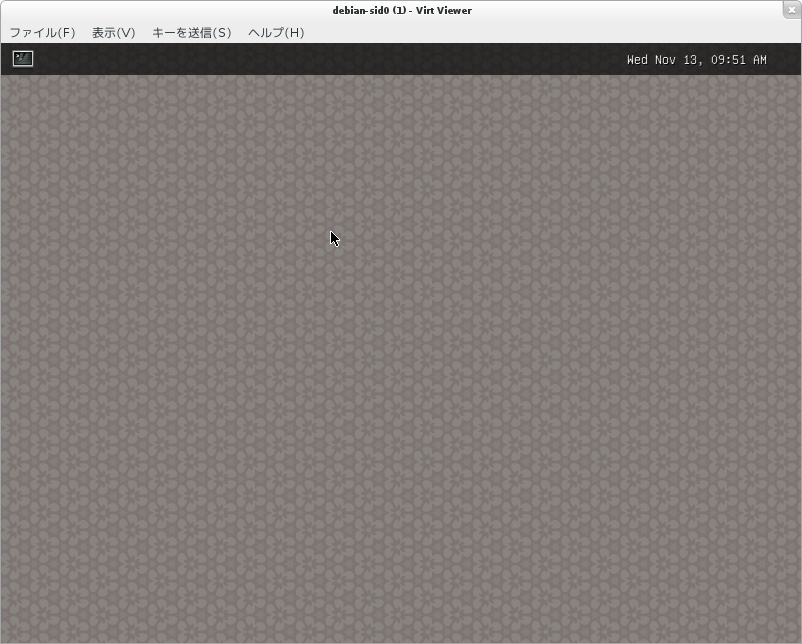
\includegraphics[width=0.8\hsize]{image201311/weston-1st-launch.png}
\end{minipage}
\begin{minipage}{0.5\hsize}
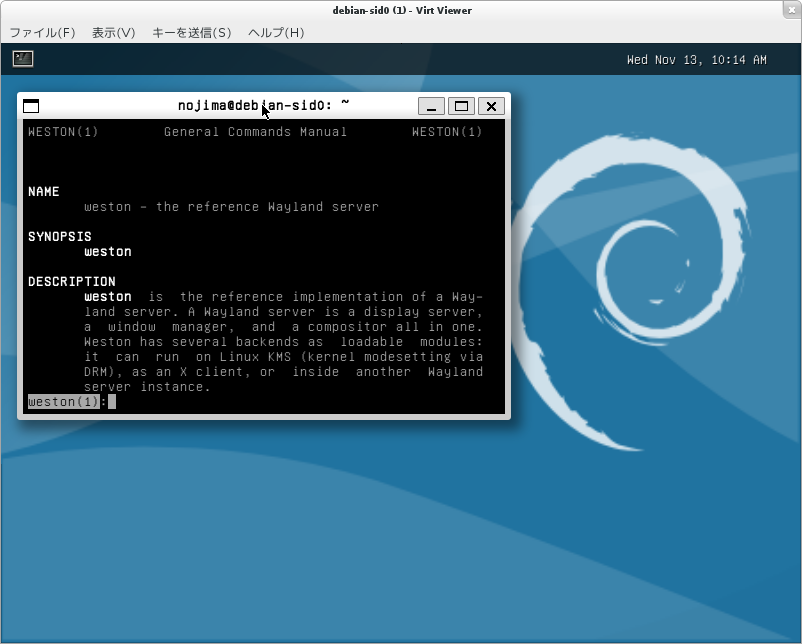
\includegraphics[width=0.8\hsize]{image201311/weston-2nd-launch.png}
\end{minipage}

\subsection{westonの対応出力デバイス}

 westonの対応できる出力デバイスは表\ref{tab:debian-weston-backends}となります。

\begin{table}[ht]
\begin{center}
\begin{tabular}{|l|p{4cm}|p{4cm}|p{3cm}|l|}
\hline 
項番&出力デバイス&バックエンド名&パッケージに搭載済&備考\\
\hline \hline
1& DRM/KMS & drm-backend.so & ○ & \\
2& FrameBuffer & fbdev-backend.so & ○ & \\
3& X & x11-backend.so & ○ & \\
4& Wayland & wayland-backend.so & ○ & \\
5& Headless & headless-backend.so & ○ & \\
5& Rassberry Pi & rpi-backend.so & × & \\
6& RDP & rdp-backend.so & × & \\
\hline
\end{tabular}
\label{tab:debian-weston-backends}
\caption{出力デバイスとwestonの対応状況}
\end{center}
\end{table}

\subsection{debianでのweston稼働のための下準備}
\label{sec:pre-requisite}
debianでwestonを動作させるには、以下の下準備が必要です。

\begin{description}
\item [Step 1.] westonの導入をします。
\begin{commandline}
# aptitude install weston
\end{commandline}
\item [Step 2.] systemdパッケージを導入するなどして、環境変数XDG\_RUNTIME\_DIRが設定されるようにします。
\begin{commandline}
# aptitude install systemd
\end{commandline}
\item [Step 3.] weston-launchにユーザを加え、ログインしなおします。
\begin{commandline}
# usermod -a -G weston-launch <your-login-id>
...重要:この後ログインしなおす...
\end{commandline}
\item [Step 4.] 環境変数XDG\_RUNTIME\_DIRが設定されているか確かめます。なお、何らかの理由で、systemdパッケージ付属のsystemd-logindが動作しない等の理由により、XDG\_RUNTIME\_DIRが設定されていないのであれば、export XDG\_RUNTIME\_DIR=/tmpなどして書き込みが可能なディレクトリを指定しておきます。
\begin{commandline}
[1] systemd-logindが無事動いている場合↓
$ env| fgrep XDG_RUNTIME_DIR
XDG_RUNTIME_DIR=/run/user/1000

[2] systemd-logindが何らかの理由で動作していない場合↓
$ env| fgrep XDG_RUNTIME_DIR
...なにも表示されない...
$ export XDG_RUNTIME_DIR=/tmp
\end{commandline}
%$
\end{description}

\subsection{その1:X上で動かしてみる}

 一番簡単に動かせます。Xのターミナルソフト上で、

\begin{commandline}
weston
\end{commandline}

とするだけで、x11-backend.soが読み込まれ、
westonの窓が開き、westonが動作を開始します。

停止する時は、westonを起動しているターミナルで、Ctrl-Cを押下します。

\subsubsection{X上で動かしてみる時の注意点}

 何故か、手元のnvidia製グラフィクスカードにて、non-freeのnvidiaドライバを
使っていると、画面真っ黒のウィンドウが開いてしまいました。--use-pixmapを指定
してwestonを起動して、westonがEGL等のハードウェアアクセラレーションを
利用しないようにしても同様だったりします。一方で、intel製のグラフィクス
チップを載せているノートPC上では問題なく動作しました。

 こちらの原因はまだつかめていません。

\subsection{その2:KMS/DRMで動かしてみる}

 intelのグラフィックスチップが搭載されているPC(例:ノートPCとか)
であれば、linuxのKMS/DRMドライバで動作します。また、
AMD/Nvidiaのグラフィクスチップであれば、linuxのKMS/DRMドライバの
radeon/nouveauドライバで動作すると思われますが、自分は未評価です。
どなたかradeon/nouveauで動作した方がいらっしゃれば教えてください。

\begin{description}
\item [Step 1.] グラフィカルなログイン画面が出ているようであれば、こちらを停止させます。\\
例:gdm3が立ち上がっている場合の止め方
\begin{commandline}
Ctrl-Alt-F1等を押下してコンソールに切り替える
$ su
# service gdm3 stop
\end{commandline}
%$
\item [Step 2.] KMS/DRMドライバが有効であることを確かめます。
\begin{commandline}
$ lsmod | egrep '(i915|radeon|nouveau)'
...(i915/radeon/nouveauのどれかの文字列が出ればOK)...
\end{commandline}
%$
\item [Step 3] westonを動かします。
\begin{commandline}
$ weston-launch
\end{commandline}
%$
\end{description}

\subsubsection{KMS/DRM上で動かしてみる時の注意点}

 linuxのKMS/DRMドライバは、i915/radeon/nouveau以外は動作するかどうかは正直やってみないと分かりません。

 例えば、debianにて、仮想化技術のKVMではcirrusチップセット用のKMS/DRMドライバがvirt-viewerの元で使えるのですが、westonはegl側cirrus未対応によるエラーもしくは、Segfaultで落ちてしまうためどうにも動作しませんでした。こちらも原因が自分では正確につかめていません。

\subsection{その3.FrameBufferデバイス上で動かしてみる}

 linuxのFrameBufferデバイス上で動かしてみます。今のところ仮想化技術のKVM上で動かすのに便利です。ここでは、実際にKVMを使って動かします。

 なお、大変残念なことに、現在のdebian sidで導入できるwestonパッケージのバージョン1.3.0では、仮想端末制御に関するupstream側のバグのために、FrameBufferデバイスでは動作しません。幸い、こちらのバグが修正された、weston-1.3.1がリリースされましたので、ここでは、このバージョンを簡易的にdebianパッケージ化して導入します。

\begin{description}
\item [Step 1.]  westonを動かす対象のdebian sidをKVMを使ってインストールします。なお、KVMホストOS側のdebian機のbr0はインターネットに接続できるように設定されているものとします。br0のセットアップについて、詳しくは\cite{kde-devel-debian}を参照してください。
\begin{commandline}
# aptitude install libvirt-bin virtinst
# qemu-img create -f raw /var/lib/libvirt/images/debian-sid0 10G
# wget http://cdimage.debian.or.jp/7.2.0/multi-arch/iso-cd/debian-7.2.0-amd64-i386-netinst.iso
# virt-install --connect=qemu:///system -n debian-sid0 --ram 512  --cdrom /home/yours/debian-7.2.0-amd64-i386-netinst.iso \
  --disk /var/lib/libvirt/images/debian-sid0,bus=virtio,size=10,format=raw,cache=writeback \
  --bridge=br0,model=virtio --vnc --hvm --accelerate
\end{commandline}

 なお、インストールの際の設定は表\ref{tab:inst-settings}のとおりを仮定します。

\begin{table}[ht]
\begin{center}
\begin{tabular}{|l|p{5cm}|p{7cm}|l|}
\hline 
項番&設定項目&指定内容&備考\\
\hline \hline
1&select a language& Japanese& \\
2&場所の選択&日本&\\
3&ネットワークの設定&手動設定。 IP:192.168.0.2, Netmask:255.255.255.0, Gateway:192.168.0.1, Host名:debian-sid0& \\
4&パッケージマネージャの設定&ミラー:日本,ミラーサイト:ftp.jp.debian.org, HTTPプロキシ:空欄&\\
5&ソフトウェアの選択&SSHサーバー、標準システムユーティリティのみ選択。あとはすべて解除。& \\
\hline
\end{tabular}
\caption{\label{tab:inst-settings}インストーラで選択する項目}
\end{center}
\end{table}

\item [Step 2.] インストール完了したら、すぐにdebian sidへアップグレードします。

\begin{commandline}
debian-sid0にログインの後、
debian-sid0 $ su
debian-sid0 # cat > /etc/apt/sources.list
deb http://ftp.jp.debian.org/debian/ sid main contrib non-free
deb-src http://ftp.jp.debian.org/debian/ sid main contrib non-free
<ctrl+d>を押下
debian-sid0 # aptitude update;aptitude full-upgrade;aptitude clean
\end{commandline}
%$

\item [Step 3.] weston-1.3.1-1パッケージを作って導入します。

\begin{commandline}
debian-sid0 # aptitude build-dep weston/sid
debian-sid0 # aptitude install libxcb-composite0-dev fakeroot
debian-sid0 # exit
debian-sid0 $ mkdir weston weston-work
debian-sid0 $ cd weston
debian-sid0 $ apt-get source weston/sid
debian-sid0 $ cd ../weston-work
debian-sid0 $ wget -O weston_1.3.1.orig.tar.gz \
  http://cgit.freedesktop.org/wayland/weston/snapshot/weston-1.3.1.tar.gz
debian-sid0 $ tar xzf weston_1.3.1.orig.tar.gz
debian-sid0 $ cd weston-1.3.1
debian-sid0 $ tar xzf ../../weston/weston_1.3.0-1.debian.tar.gz
debian-sid0 $ cd debian; 
debian-sid0 $ patch -p1 <<__HERE
--- debian.org/changelog        2013-10-11 20:04:50.000000000 +0900
+++ debian/changelog    2013-11-12 14:48:36.219299000 +0900
@@ -1,3 +1,9 @@
+weston (1.3.1-1) unstable; urgency=low
+
+  * update to upstream
+
+ -- your name <foo@bar.com>  Fri, 11 Nov 2013 12:34:56 +0900
+
 weston (1.3.0-1) unstable; urgency=low
 
   [ Sven Joachim ]
diff -ru debian.org/control debian/control
--- debian.org/control  2013-10-11 19:58:17.000000000 +0900
+++ debian/control      2013-11-12 14:49:32.347299000 +0900
@@ -35,6 +35,7 @@
  libpam0g-dev,
  libvpx-dev,
  libsystemd-login-dev,
+ libxcb-composite0-dev,
 Standards-Version: 3.9.4
 Homepage: http://wayland.freedesktop.org/
 Vcs-Git: git://anonscm.debian.org/pkg-xorg/wayland/weston
__HERE
debian-sid0 $ cd ..
debian-sid0 $ env DEB_BUILD_OPTIONS='noopt nostrip' \
   dpkg-buildpackage -rfakeroot -us -uc 2>&1 | tee ../build.log
debian-sid0 $ cd ..
debian-sid0 $ su
debian-sid0 # dpkg -i ./weston_1.3.1-1_amd64.deb
\end{commandline}

\item [Step 3.]  \ref{sec:pre-requisite}章のStep 2.〜Step 4.に記載の下準備をしておきます。(Step 1.は先ほど構築したwestonパッケージが導入済みですので不要です)


\item [Step 4.] FrameBufferのセットアップをします。なおwestonを動かすためには、color depthは24bitでなければなりません。
\begin{commandline}
debian-sid0 # aptitude install fbset
debian-sid0 # modprobe cirrusfb
debian-sid0 # fbset -g 800 600 800 600 24
\end{commandline}

\item [Step 5.] 一般ユーザになり、westonを起動します。
\begin{commandline}
debian-sid0 # exit 
debian-sid0 $ weston-launch -- --backend=fbdev-backend.so --log=weston.log
\end{commandline}
%$
\end{description}

\subsection{westonのカスタマイズ}

 westonはデフォルトのままだと少し寂しい画面なので、ちょっとカスタマイズしてみます。カスタマイズは$HOME/.config/weston.iniにいろいろ記載すると、いろいろとカスタマイズできます。ここでは壁紙を入れ、ウィンドウポップアップがアニメーションするようなカスタマイズをしてみます。
\begin{commandline}
$ cat >.config/weston.ini <<__HERE 
[shell]
background-image=/usr/share/images/desktop-base/spacefun-grub.png
background-type=tile
locking=true
animation=zoom
binding-modifier=ctrl

[launcher]
icon=/usr/share/weston/terminal.png
path=/usr/bin/weston-terminal
__HERE
\end{commandline}
%$

\subsection{westonの構造}

 図\ref{fig:wayland-internal}にwaylandアプリケーションとwestonの構造を載せます。

\begin{figure}[H]
\begin{center}
 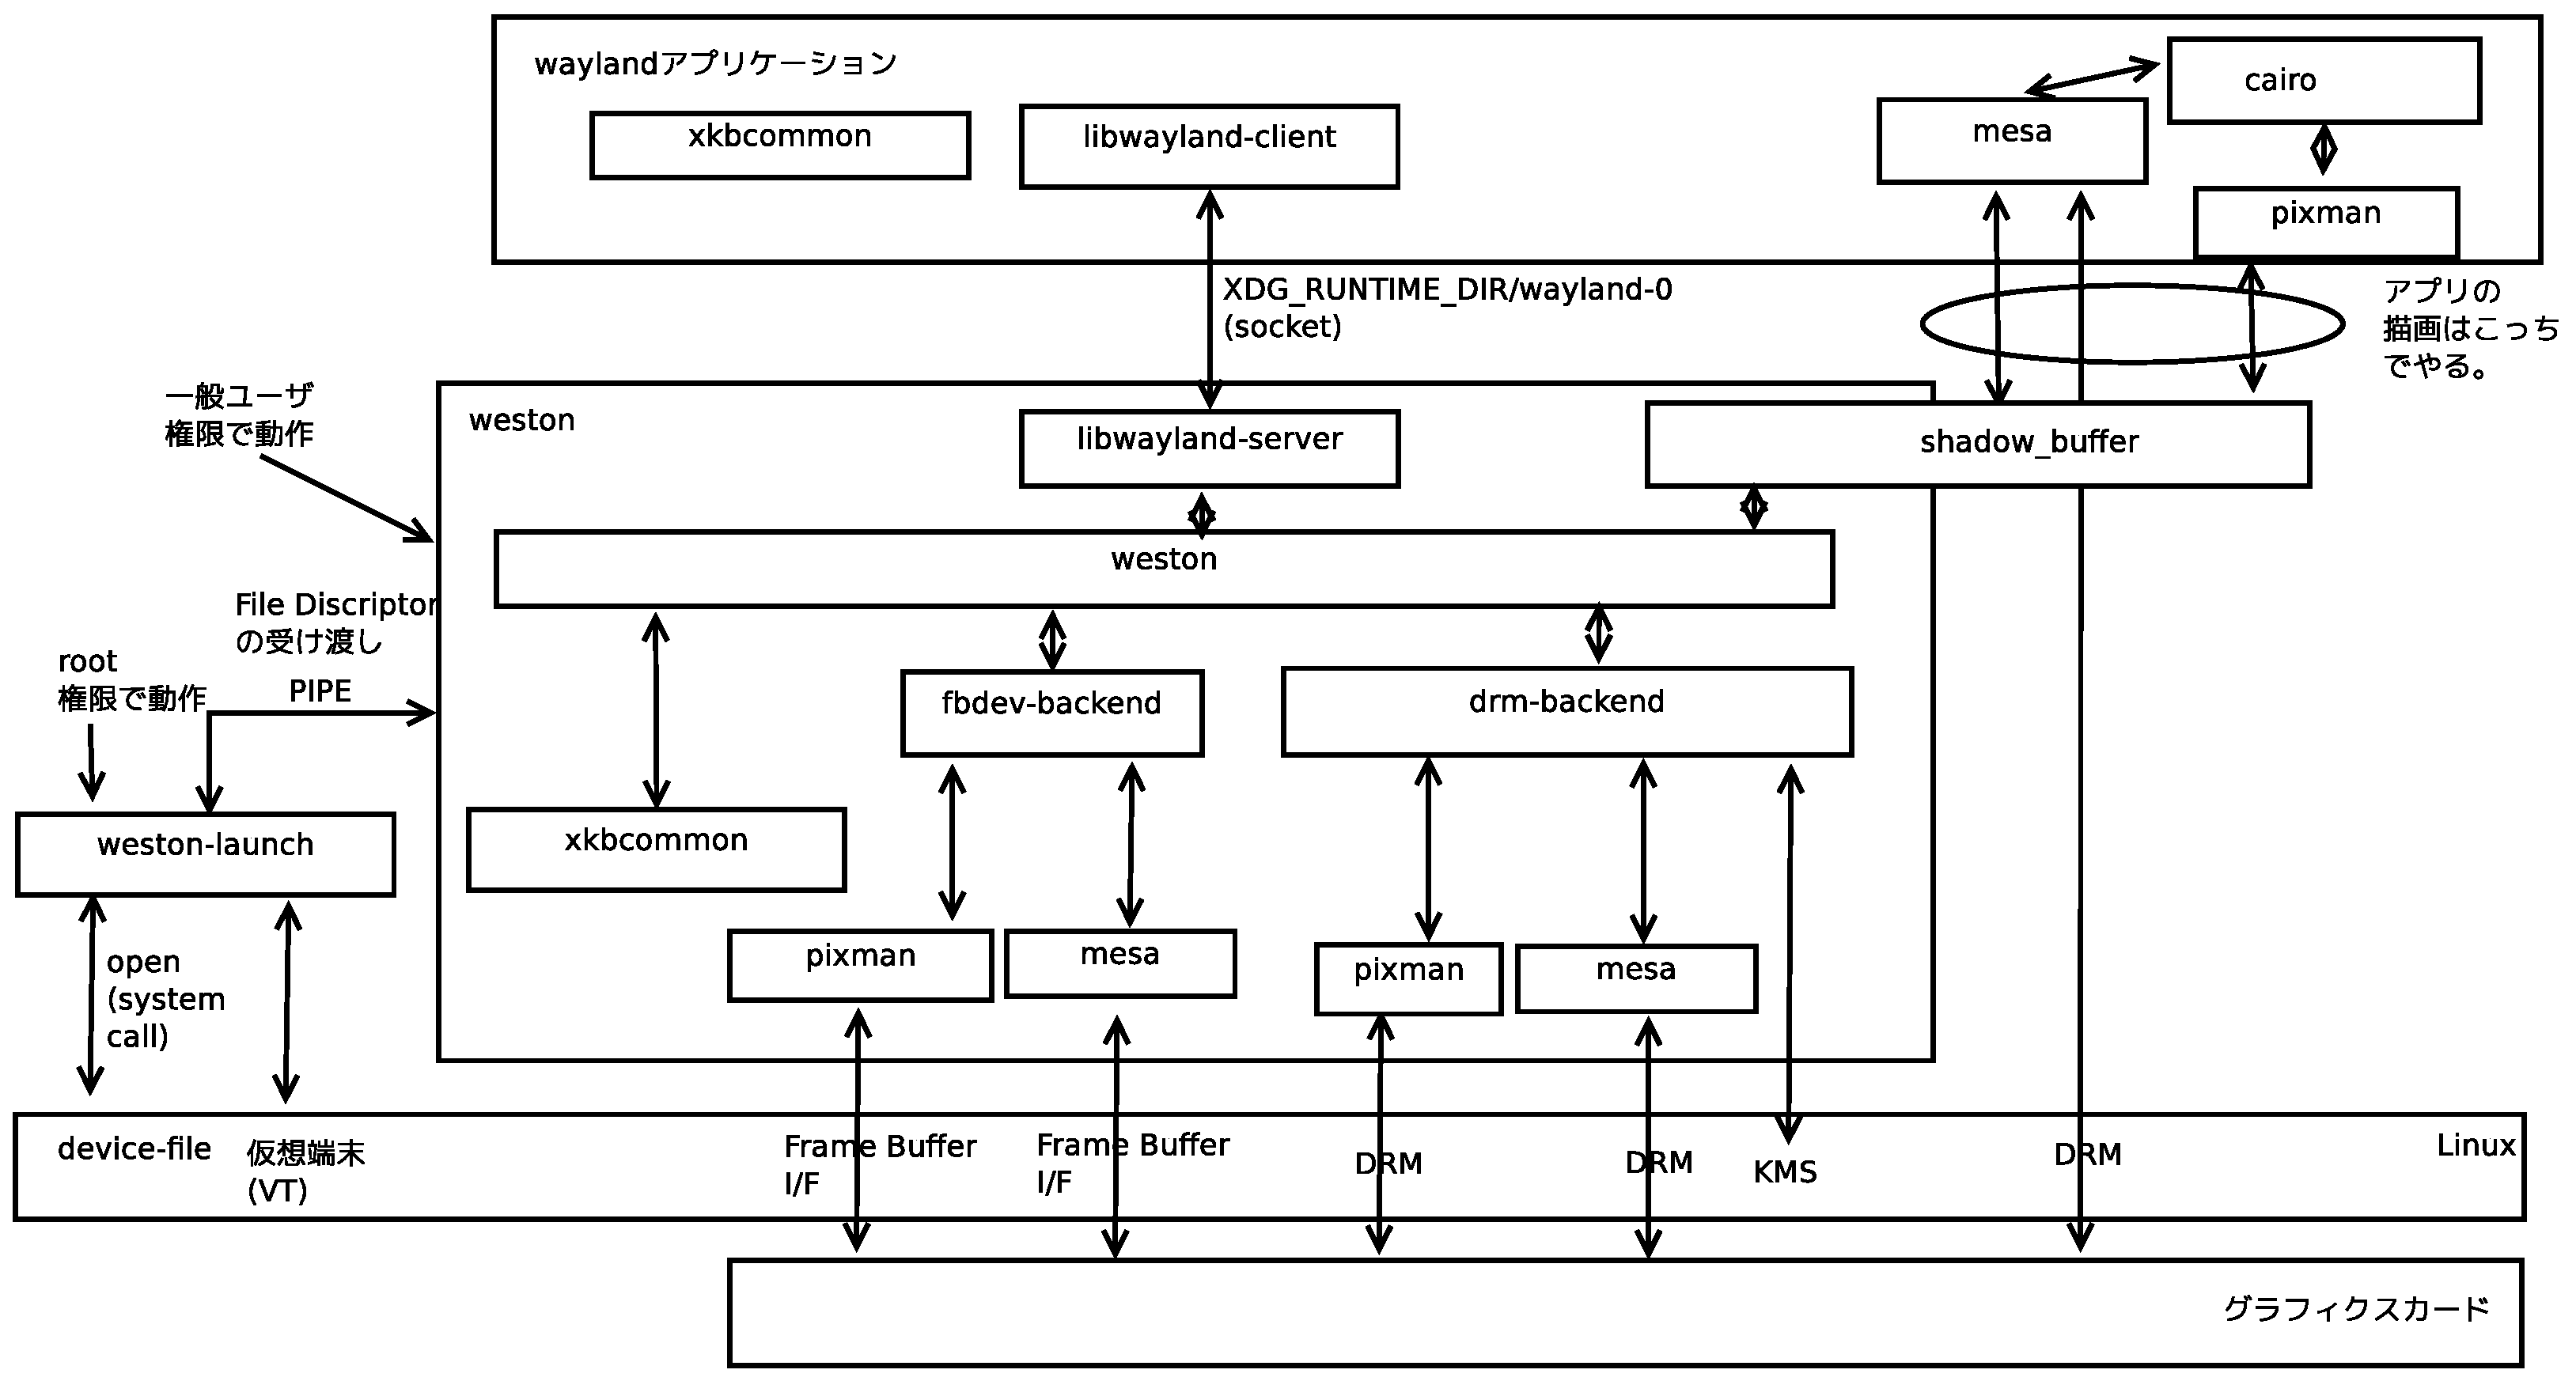
\includegraphics[width=0.8\hsize] {image201311/wayland-internal-schema.eps}
 \caption{waylandアプリケーションとweston}
\label{fig:wayland-internal}
\end{center}
\end{figure}

 特徴として、
\begin{itemize}
\item 基本的にアプリケーション側も含めて、ローカルシステムで描画を行うことを前提にした作りになっています。
\item cairo/mesa/xkbcommon等を最大限利用して、weston自体は非常にシンプルな設計になっています。
\item プロセスのユーザ権限を制限するため、weston-lanchにはroot権限が最低限必要な部分のみの操作を、westonは一般ユーザでの権限による動作をするように、権限が分割されています。なお、現在の実装ではweston-launchは操作・オープン済みの端末のFileDiscriptorと、デバイスファイルのFile Descriptor、weston-launchへのシグナルを、westonの求めに応じて引き渡す機能が実装されています。
\end{itemize}
\subsection{その他}

 debianで利用できるweston/waylandにはちょっとしたクセがあります。

 \begin{itemize}
\item Xwaylandが動作しません。これはwestonが起動するXにwayland用のI/Fを搭載するパッチが摘要されていなければならない(X起動時に-waylandオプションが使えなければならない)のですが、こちらは未だXのパッケージに含められていない為となります。なお、2013/10頃にこちらのdebianパッケージ用のパッチがdebian-xのMLに流れていました。
\item gtk等の有名なツールキットはwayland未対応の状態です。
 \end{itemize}

\subsection{おわりに}

 次期ディスプレーサーバーになるかもしれないwestonとwaylandについて、いろいろ試してみました。プログラム本体は非常に小さいプログラムですし、発展途上ですので、いじってみようという方は、今ならたやすく改造/解析し放題の旬な時です。Hackの対象にぜひ。

\begin{thebibliography}{0}
  \bibitem{real-wayland-X}
    {\footnotesize{
       Daniel Stone,``The real story behind Wayland and X'',linux.conf.au 2013,
       \url{http://people.freedesktop.org/~daniels/lca2013-wayland-x11.pdf},
       \url{http://www.youtube.com/watch?v=RIctzAQOe44}
       }}
  \bibitem{kde-devel-debian}
    {\footnotesize{
       野島 貴英,「Debian開発者のKDE環境あれこれ」,第85回東京エリアDebian勉強会資料,
       \url{http://tokyodebian.alioth.debian.org/pdf/debianmeetingresume201202.pdf}
       }}
\end{thebibliography}

%-------------------------------------------------------------------------------
\dancersection{tramp入門}{上川純一}
%-------------------------------------------------------------------------------
\index{tramp}
\index{emacs}

\subsection{emacsでリモートファイル編集するTrampのすすめ}

リモートサーバでファイルの編集はどうしていますか?moshを使っている?
sshfsを使っている?いろいろあると思いますがmoshを使うとローカルのファイル
と扱いが変わってしまい、リモートのviだったりemacsを使って編集することにな
り、設定の同期がほぼ不可能になります。一方sshfsだとローカルファイルのよう
に扱うことができるのですが、rootなどの別のユーザ(root?)としてファイルの
編集ができにくかったりしますし、リモートホストでコマンドを実行しようとす
ると別途sshでログインして作業することになり、sshセッションをひらきながら
sshfsで実行し、ローカルのパスとリモートのパスの違いを意識しながら作業す
ることになります。

emacs ユーザの方々に朗報です。tramp とは \texttt{/sshx:hostname:path/to/file} とい
う特殊なファイル名を指定すると透過的にsshを使ってリモートのファイルを取
得して編集できるようにしてくれる仕組みです。
また、dired でリモートのディレクトリのファイル管理もローカルと変わらない
ように行えます。
さらに便利なのは \texttt{M-x shell}, \texttt{M-x compile} などリモートでコマンドを実行する
コマンドを利用するとhostname にsshでログインして path/to/file をカレント
ディレクトリとした状態でコマンドを実行してくれるところです。
個人的にはmoshなどを利用してシェルのコマンドを実行するより、emacsのロー
カルバッファでコマンドラインを編集して確定時にリモートに送信するスタイル
が気に入っています。

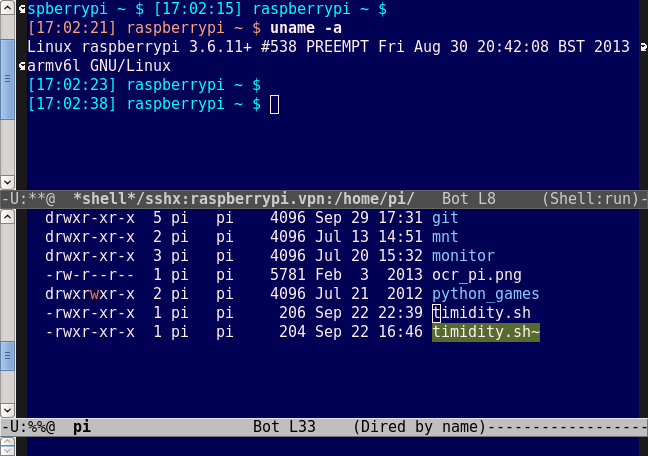
\includegraphics[width=12cm]{image201311/tramp-screenshot.png}


\subsection{リモートホスト側の設定}
ssh で接続される側のの設定ですが、trampはシェルのセッションの入出力を利用し、機械的に
プロンプトを検出するので、プロンプト(PS1など)をカスタマイズしていると
動かない場合があります。trampのために \texttt{.bashrc}はシンプルにするといいかも
しれません。

例えば、raspbian のデフォルトは色がつきまくってたりしてファンシー過ぎてう
まく動きませんでした。

\subsection{sshの設定とチューニング}
\index{ssh}
\index{ssh\_config}

ローカルのsshの設定ファイル \verb!~/.ssh/config! に設定したほうがよいも
のを紹介します。
マニュアルは \verb!man ssh_config!\cite{sshconfig}で参照できます。

\subsubsection{ControlMasterで接続を再利用}

手元ではこんな設定にしています。

\begin{commandline}
 ControlMaster auto
 ControlPersist 120
 ControlPath ~/tmp/ssh-%r@%h:%p
\end{commandline}


ControlPersist に指定した秒数間、sshで接続する際にデーモンプロセスが起動
して、コネクションを張りっぱなしにし、コネクションを再利用してくれます。

手元では、ControlPathを明示的に指定しています。ホームディレクトリ以下の
tmp 以下にしているのはファイル名が予想可能になるので衝突を防ぐためです。

ControlMasterをAutoにしておくとすでにコネクションが開いていない場合はデー
モンをたちあげて、もしコネクションが開いている場合にはそれを利用するよう
になります。

リモートでtrueコマンドを実行する速度を計測してみたところ
随分高速になり(\fgref{fig:pingwagner})、ping time の二倍くらいになってくれ
るようです。

\begin{table}[ht]
\begin{center}
  \begin{tabular}{|c|c|}
   command & time(ms) \\
   ping& 271 \\
   ssh connection sharing on & 544 \\
   ssh connection sharing off & 4070 \\
 \end{tabular}
 \caption{ping test against wagner.debian.org}
 \label{fig:pingwagner}
\end{center}
\end{table}

\subsubsection{keep-alive}

trampはネットワーク接続の切断をsshプロセスの生死で検出します。
sshはネットワーク接続がきれたりしてもすぐにはそれを検出しないので、キー
プアライブを送信するようにします。

\begin{commandline}
 ServerAliveInterval 3
 ServerAliveCountMax 5
\end{commandline}


本当はパソコンがサスペンドから復活して新しいネットワーク接続につながった
らsshプロセスに再接続してほしいのですが、その方法をまだ発見できていませ
ん。

\subsubsection{その他の設定}

Mac のRendezvousとかLinuxのAvahiとか設定しているとホスト名.local という名
前で名前解決ができるようになりますが、そうするとIPアドレスはDHCPだと一定
ではないため、IPに対しての鍵が違うと怒られます。その場合はホストIPをチェッ
クしないようにするとよいでしょう。

\begin{commandline}
 Host *.local
  CheckHostIP no
\end{commandline}

あとデフォルトではいろいろな鍵を試したりする設定になっていますが、ついで
に鍵を指定して公開鍵認証にしておくとよいんじゃないでしょうか。

\begin{commandline}
 Host tekitouna.vpn
  Hostname そのホストのIPアドレス
  IdentityFile ~/.ssh/ssh-keygenで作ったファイルのパス
  IdentitiesOnly yes
\end{commandline}


\subsection{trampの.emacs での設定とチューニング}

\texttt{.emacs} にほとんど設定しなくてもデフォルトの設定でそれなりにうご
きます。
マニュアルは info 形式で提供されています\cite{trampinfomanual}。

trampでは\texttt{/sudo:root@hostname:/} のような形式でリモートホスト上で
sudoで別ユーザになってからファイルにアクセスするように指定することが可能
です。ただ、そのためにはリモートホストへの到達手段を指定する必要がありま
す。たとえば、ローカルネットワークにあるホスト \texttt{*.local} でsudoを
サポートしたいという要望であれば、次のような設定を追記しておきます。

\begin{commandline}
 (add-to-list 'tramp-default-proxies-alist
      '("\\.local\\'" "\\`root\\'" "/ssh:%h:"))
\end{commandline}

あと、デフォルトの設定だとリモートアクセスしているというメッセージがステー
タスに表示されるのですが、正直邪魔なのでそれを消すのもよいかと思います。

\begin{commandline}
(custom-set-variables '(tramp-verbose 1))
\end{commandline}

\begin{thebibliography}{0}
 \bibitem{trampinfomanual} ``TRAMP User Manual'', info
	 page,
	 \url{http://www.gnu.org/software/emacs/manual/html_node/tramp/index.html#Top}
 \bibitem{sshconfig} ``ssh\_{}config(5)'' manual page,
\end{thebibliography}

\printindex

\cleartooddpage

\vspace*{15cm}
\hrule
\vspace{2mm}

\includegraphics[width=2cm]{image200502/openlogo-nd.eps}
\noindent \Large \bf Debian 勉強会資料\\
\noindent \normalfont \debmtgyear{}年\debmtgmonth{}月\debmtgdate{}日 \hspace{5mm}  初版第1刷発行\\
\noindent \normalfont 東京エリア Debian 勉強会 (編集・印刷・発行)\\
\hrule

\end{document}
